\textcolor{blue}{Problem 3}
According to the iterative format provided as follow:
\begin{itemize}
    \item Use the SUV dataset to implement (using Python or MATLAB) the Gradient Descent method to find the optimal model for logistic regression.
    \item What is your test error? What are the sizes of the training set and test set, respectively?
    \item What is your learning rate? How was it chosen? How many steps were iterated in total?
    \item Present the results of the last 10 steps produced by your algorithm, including the loss, learning rate, the L2 norm of the gradient, and the number of function evaluations and gradient evaluations.
\end{itemize}
\begin{figure}[htbp]
\centerline{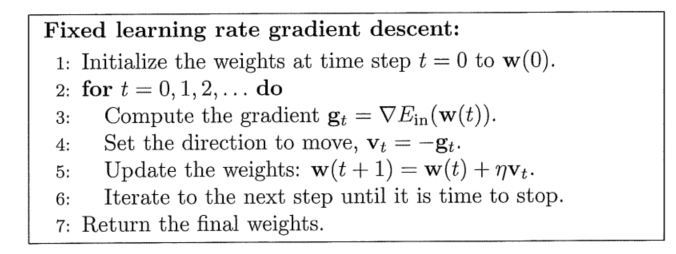
\includegraphics[width=0.8\textwidth]{./image/alg.png}}

\href
  {https://www.cs.toronto.edu/~mhsadi/code-repository/MachineLearningNotebooks/3-SUVDataset.html}
  {Dataset reference and description}
  \\
\href
{https://www.kaggle.com/datasets/iamaniket/suv-data?resource=download}
  {Dataset and download}

\end{figure}

\textcolor{blue}{Solution}

After checking the SUV dataset, we could find that each buyer's information has a unique `User ID', so we can just drop the `User ID' column.\\
To use the `Gender' information, we map `Male' into $1$, and `Female' into $0$.\\
Then the `Gender', `Age', `EstimatedSalary' can be used as the input features, and the `Purchased' can be used as the output label.\\
So this is a binary classification problem.\\
And we can use the logistic regression to solve this problem.\\

1. Since we are applying the logistic regression, so the testing error is:
$$E_{\text {in }}(\mathbf{w}) = \dfrac{1}{N}\sum_{i=1}^{N}\log (1+e^{-y_n\mathbf{w}^T\mathbf{x}_n})$$
which have been proved in Problem 1. And $N$ is the size of the testing set's size.\\

The size of training set is ? persent, which is totally ? samples. And the testing set is ? persent, which is totally ? samples.\\

2. We have known that the gradient of logistic regression from Problem 1 is:
$$\nabla E_{\text {in }}(\mathbf{w}) = \dfrac{1}{N}\sum_{i=1}^{N}-y_n\mathbf{x}_n\theta(-y_n\mathbf{w}^T\mathbf{x}_n)$$

So the learning rate is set to be
$\eta = 0.1$
$\eta_t = \eta\cdot \|\nabla E_{\text{in}}(\mathbf{w})\|$

And the total iterated steps is 


3. The results of the last 10 steps are shown as follow:



TODO:
1. last 10 steps' output
2. loss against iteration, gradient norm against iterataion, stepsize against iteration
3. AUC, ROC curve







